\documentclass{ximera}
\typeout{Start loading xmPreamble.tex}%

% Add here extra macro's that are loaded automatically by all documents of claas 'ximera' or 'xourse' in this repo

%%
%%  Example:
%%
% \newcommand{\R}{\mathbb{R}}
\usepackage{tikz}
\usetikzlibrary{positioning, arrows.meta}
\usepackage{multicol}
\usepackage{enumitem}
\usepackage{caption}
\usepackage{amsmath}
\usepackage{amsthm}


\title{Markov Chains and Processes On Discrete State Spaces}
\begin{document}
\begin{abstract}
\end{abstract}
\maketitle

Consider a simple random walk on a ring.
\vspace{1cm}

\begin{figure}[h]
\begin{center}
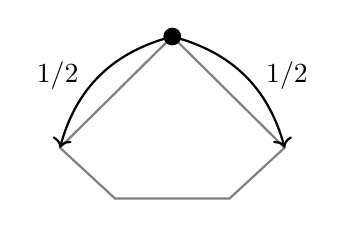
\begin{tikzpicture}[scale=1.5]
% Pentagon vertices (top vertex first, going clockwise)
\coordinate (A) at (90:1.25);     % top
\coordinate (B) at (18:1);        % upper right
\coordinate (C) at (-14:.5);      % lower right
\coordinate (D) at (194:.5);      % lower left
\coordinate (E) at (162:1);       % upper left

% Draw pentagon edges in gray (no filled nodes)
\draw[gray, thick] (A) -- (B) -- (C) -- (D) -- (E) -- (A);

% Filled dot only at top vertex
\filldraw[black] (A) circle (2pt);

% Curved arrows from top vertex to adjacent vertices
\draw[->, thick, bend right=30] (A) to node[left, xshift=-4pt] {$1/2$} (E);
\draw[->, thick, bend left=30]  (A) to node[right, xshift=4pt]  {$1/2$} (B);
\end{tikzpicture}

\xmalt{Image of a simple random walk on a ring with five lattice sites.}
\caption{The simple random walk on a ring with five lattice sites.}
\label{markov-ring}
\end{center}
\end{figure}

In this example, there are five lattice sites on a ring. At each time step, a particle jumps to an adjacent
site with probability $1/2$. We let $X_t$ denote the position of the particle at time $t$, where $t$ takes
values in the non-negative integers. The key property is that $X_{t+1}$ only depends on $X_t$, not on
$X_{t-1}, \ldots, X_0$. Colloquially, we say that

\begin{center}
\textit{``the future only depends on the present, not on the past.''}
\end{center}

\begin{definition}
A \textbf{Markov chain} on a (discrete) state space $\mathcal{X}$ is a sequence of random variables
$X_1, X_2, \ldots$ such that for all $k \geq 0$ and all times $t_0 < t_1 < \cdots < t_k < t$ and all states
$x_0, x_1, \ldots, x_k, x_t \in \mathcal{X}$, we have
\[
P(X_t = x_t \mid X_{t_k} = x_k,\, X_{t_{k-1}} = x_{k-1},\, \ldots,\, X_{t_0} = x_0)
= P(X_t = x_t \mid X_{t_k} = x_k).
\]
\end{definition}

Colloquially, we view $t$ as the future time, $t_k$ as the present time, and $t_0, \ldots, t_{k-1}$ as the
past times. This Markov property essentially states that the knowledge of the states at past times are
irrelevant.

This definition does not apply very well to arbitrary state spaces $\mathcal{X}$, since the probability of
being exactly in an infinitesimally small state is often zero. I will address this later.

\begin{definition}
Given a Markov chain $(X_t)$, the \textbf{transition probabilities} are defined by
\[
p_{xy}(t) = P(X_{t+1} = y \mid X_t = x)
\]
where $x, y$ are states in $\mathcal{X}$ and $t$ is any time. If $p_{xy}(t)$ does not depend on $t$, we say
that the Markov chain is \textbf{time-homogeneous} and we simply write $p_{xy}$, dropping the dependence
on $t$.
\end{definition}

I have never considered a non time-homogeneous Markov chain my entire research career. This is not to
say that those are unimportant, but rather saying that it is possible to have a research career with only
time-homogeneous Markov chains. It is an exercise to the reader to determine if I have had a good research
career.

\begin{definition}
The \textbf{transition matrix} $P$ has rows and columns indexed by state space $\mathcal{X}$ and entries
$p_{xy}$, where $x$ and $y$ are states in $\mathcal{X}$.
\end{definition}

\begin{example}
In the example of the simple random walk on a ring with five lattice sites, the transition matrix is:
\[
P =
\begin{pmatrix}
0   & 1/2 & 0   & 0   & 1/2 \\
1/2 & 0   & 1/2 & 0   & 0   \\
0   & 1/2 & 0   & 1/2 & 0   \\
0   & 0   & 1/2 & 0   & 1/2 \\
1/2 & 0   & 0   & 1/2 & 0
\end{pmatrix}
\]
\end{example}

\begin{definition}
A \textbf{stochastic matrix} has nonnegative entries and rows which sum to $1$. So a transition matrix is
stochastic.
\end{definition}

Next, we will consider situations where the time takes values in the non-negative real numbers. In these
cases, there is an added layer of difficulty, which is a reflection of the fact that the positive integers have
a smallest element $1$, whereas the positive real numbers do not. In other words, for discrete-time Markov
chains, we can increment a single time update, which is not possible in continuous-time. This subtle
distinction is important enough that the terminology is different.

\begin{definition}
A \textbf{Markov process} on a (discrete) state space $\mathcal{X}$ is a collection of random variables
$\{X_t : t \geq 0\}$ such that for all $k \geq 0$ and all times $t_0 < t_1 < \cdots < t_k < t$ and all
states $x_0, x_1, \ldots, x_k, x_t \in \mathcal{X}$, we have
\[
P(X_t = x_t \mid X_{t_k} = x_k,\, X_{t_{k-1}} = x_{k-1},\, \ldots,\, X_{t_0} = x_0)
= P(X_t = x_t \mid X_{t_k} = x_k).
\]
\end{definition}

The only change in the definition is the range of values of $t$.

\begin{definition}
Given a Markov process $(X_t)$, the \textbf{transition probabilities} are defined by
\[
p_{xy}(t, s) = P(X_{s+t} = y \mid X_s = x)
\]
where $x, y$ are states in $\mathcal{X}$ and $t$ is any time. If $p_{xy}(t, s)$ does not depend on the
current time $s$, we say that the Markov process is \textbf{time-homogeneous} and we simply write
$p_{xy}(t)$, dropping the dependence on $s$.
\end{definition}

Note we cannot drop the dependence on $t$.

\begin{definition}
The \textbf{transition matrices} $\{P(t) : t \geq 0\}$ have rows and columns indexed by state space
$\mathcal{X}$ and entries $p_{xy}(t)$, where $x$ and $y$ are states in $\mathcal{X}$.
\end{definition}

I intentionally used the plural ``matrices'' to emphasize that the transition matrices depend on the time
parameter $t$.

At this point in the notes, I have not given anything to indicate that the transition matrix and matrices
are anything other than a ``bookkeeping'' tool to arrange numbers. For example, it is natural to ask if the
eigenvalues of the matrix mean anything probabilistically. Spoiler alert: it does---you can search for the
``spectral gap of a Markov chain'' to find some results. Right now, we start with something more
elementary, which is interpreting matrix multiplication in the context of probability. But first, we need a
definition:

\begin{definition}
A set of matrices $\{P(t) : t \geq 0\}$ is called a \textbf{semigroup} if $P(s + t) = P(s)P(t)$ for all
$s, t \geq 0$.
\end{definition}

Although not particularly important for probability, a semigroup (from an algebraic perspective) is a
group but without the inversion property. In this context, $P(-t)$ would not make sense because we cannot
map a Markov process backwards in time.

\begin{theorem}
The set of transition matrices of a Markov process is a semigroup.
\end{theorem}

\begin{proof}
Let $x, y \in \mathcal{X}$ be arbitrary states. We want to show that the $(x, y)$ entry of $P(s + t)$
equals the $(x, y)$ entry of $P(s)P(t)$. So, we start with
\[
p_{xy}(s + t) = P(X_{s+t} = y \mid X_0 = x)
= \frac{P(X_{s+t} = y,\, X_0 = x)}{P(X_0 = x)},
\]
which is just the definition of the transition matrices and the definition of conditional probability.
Next, we use countable\footnote{As a side note, there is a mathematical nuance that is being skipped
here, which rarely would come up in real-world applications. If the state space $\mathcal{X}$ is discrete
and uncountable, then the sum is uncountable and it is not clear how countable additivity would apply.
One would argue that in a convergent uncountable sum of non-negative numbers, all but countably many
terms are zero. However, because I am unaware of how a discrete uncountable state space could exist in
reality, I am skipping over the details here.} additivity to re-write the numerator to obtain
\[
p_{xy}(s + t) = \sum_{z \in \mathcal{X}}
\frac{P(X_{s+t} = y,\, X_s = z,\, X_0 = x)}{P(X_0 = x)}.
\]
Intuitively this says that if we know that the Markov process started at state $x$ and ended up at state
$y$ at time $s + t$, then in the intermediate time $s$ it must have been at some state. We don't know
what state it is, but summing over all possible states we must get the same probability.

Next, we again use the definition of conditional probability to conclude
\[
p_{xy}(s + t) = \sum_{z \in \mathcal{X}}
\frac{P(X_{s+t} = y \mid X_s = z,\, X_0 = x)\, P(X_s = z,\, X_0 = x)}{P(X_0 = x)}.
\]
Now, at this point we use the Markov property to conclude that
\begin{align*}
p_{xy}(s + t)
&= \sum_{z \in \mathcal{X}}
   P(X_{s+t} = y \mid X_s = z)\,
   \frac{P(X_s = z,\, X_0 = x)}{P(X_0 = x)}.
\end{align*}
Rearranging the terms, we conclude that
\begin{align*}
p_{xy}(s + t)
&= \sum_{z \in \mathcal{X}} P(X_s = z \mid X_0 = x)\, P(X_{s+t} = y \mid X_s = z) \\
&= \sum_{z \in \mathcal{X}} P_{xz}(s)\, P_{zy}(t).
\end{align*}
Finally, the usual definition of matrix multiplication tells us that the last term is the $(x, y)$ entry of
$P(s)P(t)$, as needed.
\end{proof}

One thing to observe is that in the proof, the summation in the definition of matrix multiplication is a
result of countable additivity. For non-discrete state spaces, this argument no longer works; one would
require some knowledge of measure theory.

\end{document}